\documentclass[12pt]{scrartcl}

\usepackage[utf8]{inputenc}
\usepackage[naustrian]{babel}
\usepackage{caption}
\usepackage{graphicx}
\usepackage{verbatim}
\usepackage[T1]{fontenc}
\usepackage{lmodern}
\usepackage{subcaption}
\usepackage{amsfonts}
\usepackage{listings}
\usepackage{float}

%pdfs
\usepackage{pdfpages}
\usepackage{tikz}

%page borders
\usepackage{geometry}
\geometry{left=2.5cm,right=2.5cm,top=3cm,bottom=2.5cm}

\usepackage{minted}
\setminted {
	%style=igor, %borland, autumn, vs
	encoding=utf-8,
	autogobble,
	tabsize=4,
	linenos,
	breaklines,
	keywordcase=upper,
	%escapeinside=||
	%bgcolor=bg
	%frame=single
}

\newcommand{\var}{\textit}
\newcommand{\PK}[1]{\underline{\var{#1}}}
\newcommand{\FK}[1]{\textup{FK}(#1)}

\newenvironment{relationalmodel}
  {\par\medskip
   \setlength{\arraycolsep}{0pt}%
   $\begin{array}{ r l }}
   {\end{array}$
   \par\medskip}

\newenvironment{code}{\captionsetup{type=listing}}{}

%title/footer/header values
\usepackage{titling}
\title{DES3UE Übung 3}
\author{Elias Leonhardsberger}
\date{\today{}, Hagenberg}

%footer/header
%\usepackage[automark]{scrpage2}
%\pagestyle{headings}
%\clearscrheadfoot
%\ihead{\thetitle}
%\chead{\theauthor}
%\ohead{\today}
%\cfoot{Seite \pagemark}

\begin{document}
\clearpage
\thispagestyle{empty}
\begin{tikzpicture}[remember picture, overlay]
	\node at (current page.center) {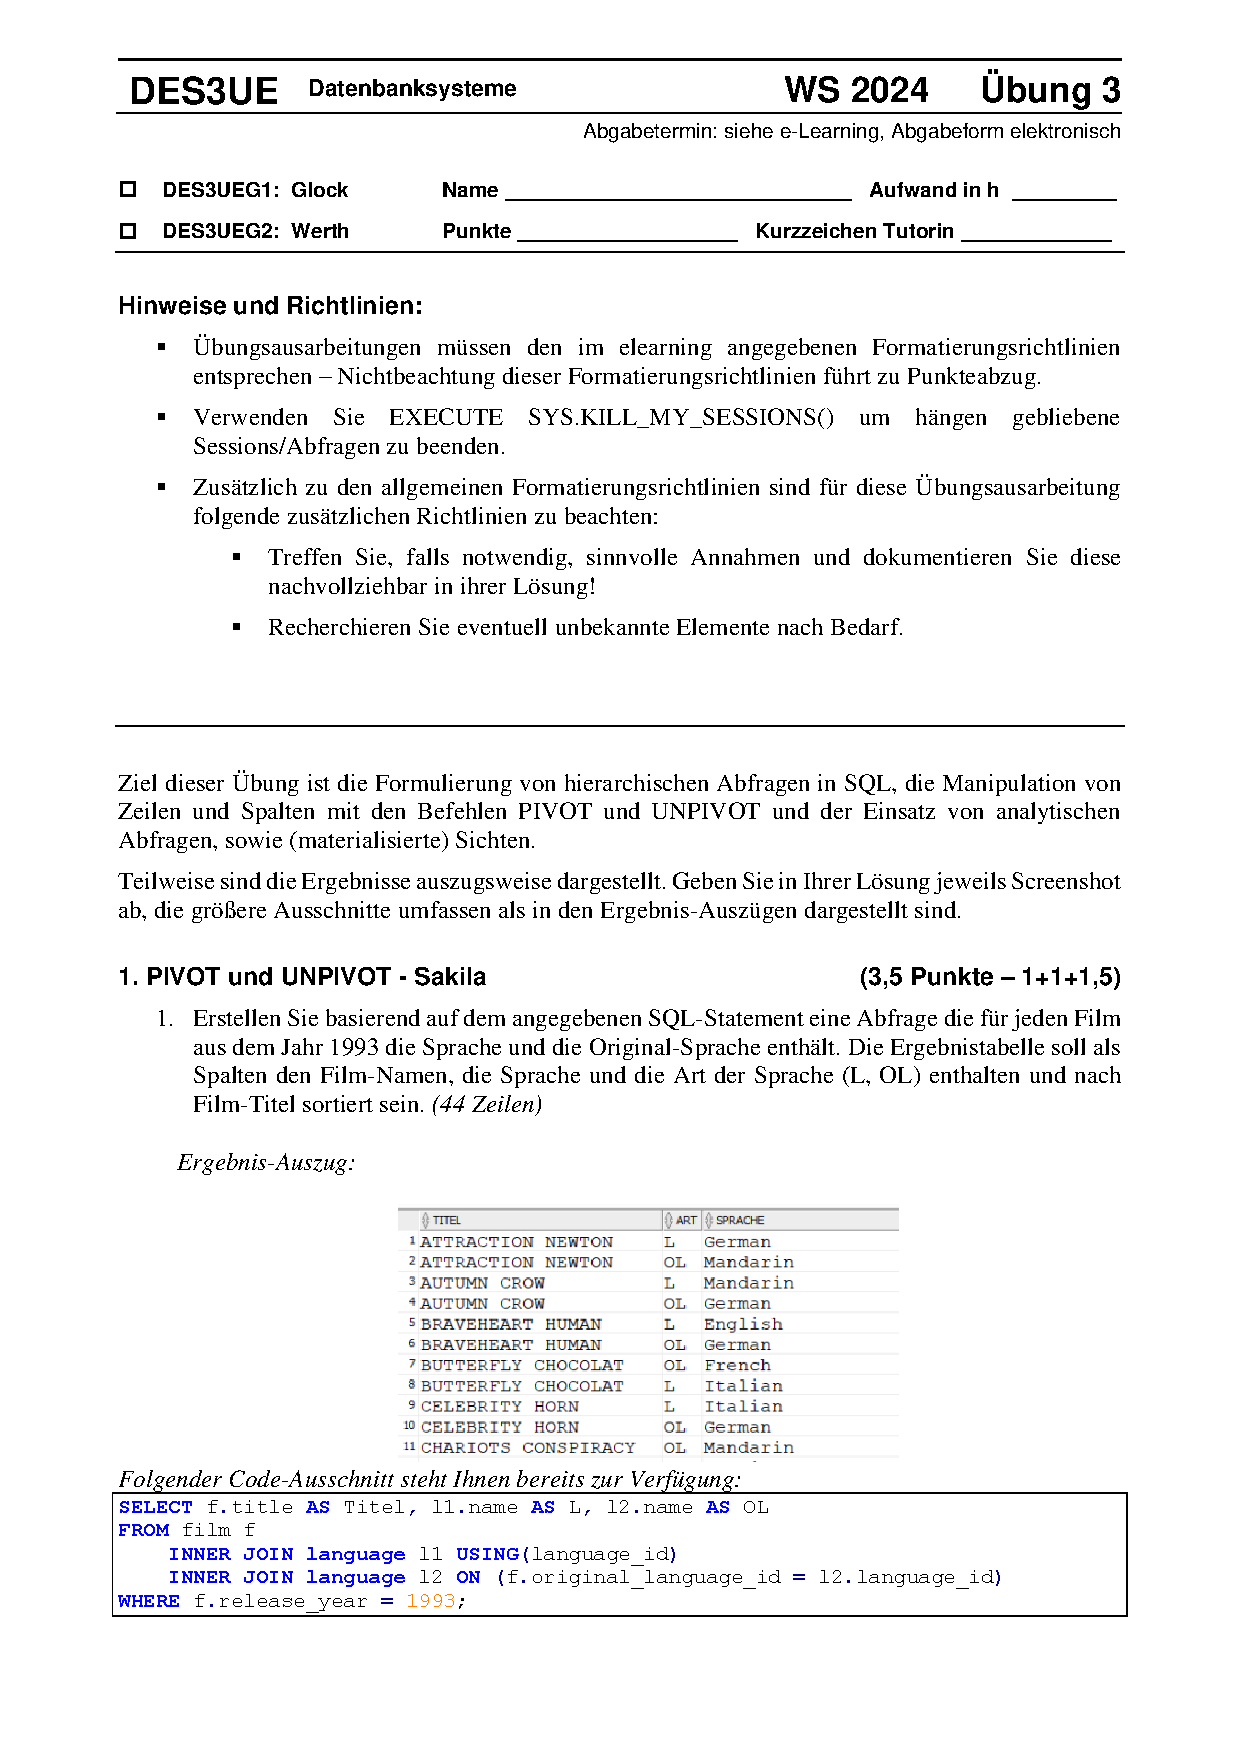
\includegraphics[page=1]{Angabe.pdf}};
	\begin{scope}[shift={(current page.south west)},every node/.style={anchor=base west}]
		\node at (8.5cm, 26.4cm) {\theauthor};
		\node at (17.2cm, 26.4cm) {6};
		\node at (1.87cm, 26.35cm) {X};
	\end{scope}
\end{tikzpicture}

\includepdf[pages=2-7]{Angabe.pdf}

\maketitle
\tableofcontents

\pagebreak

\section{PIVOT und UNPIVOT - Sakila}

\subsection{SQL Queries}
\inputminted{sql}{../ue3_1.sql}

\subsection{Ergebnisse}

\begin{figure}[H]
	\centering
	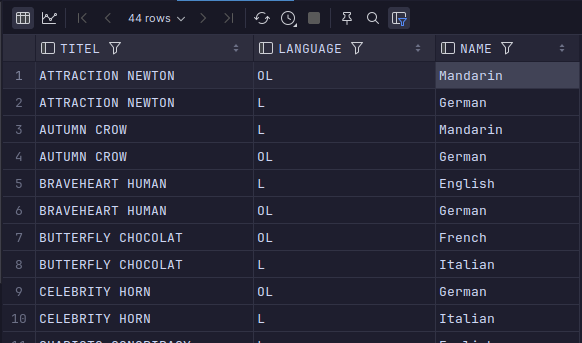
\includegraphics[width=0.7\linewidth]{../ue3_1_1.png}
	\caption{Aufgabe 1 Ergebnis 1}
\end{figure}

\begin{figure}[H]
	\centering
	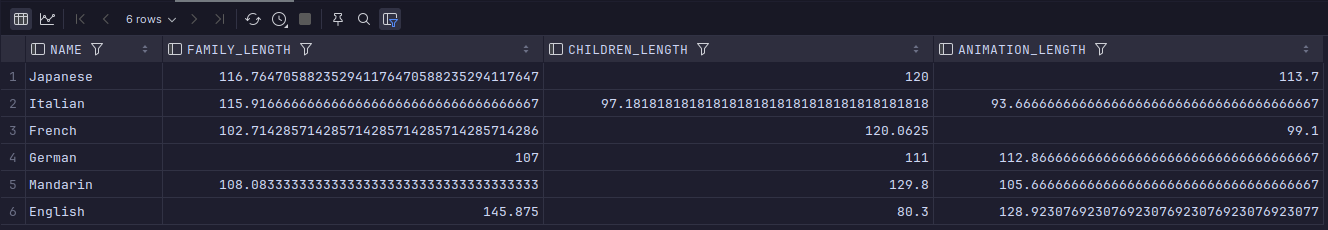
\includegraphics[width=1\linewidth]{../ue3_1_2.png}
	\caption{Aufgabe 1 Ergebnis 2}
\end{figure}

\begin{figure}[H]
	\centering
	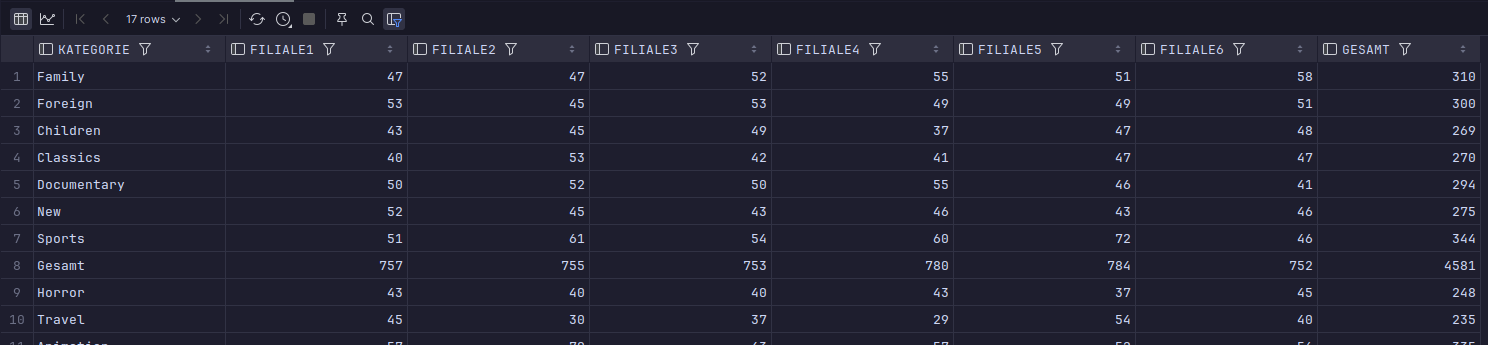
\includegraphics[width=1\linewidth]{../ue3_1_3.png}
	\caption{Aufgabe 1 Ergebnis 3}
\end{figure}

\pagebreak

\section{Hierarchische Abfragen - Human Resources}

\subsection{SQL Queries}

\inputminted{sql}{../ue3_2.sql}

\subsection{Ergebnisse}

\begin{figure}[H]
	\centering
	
\includegraphics[width=1\linewidth]{../ue3_2_1a.png}
	\caption{Aufgabe 2 Ergebnisse 1}
\end{figure}

\begin{figure}[H]
	\centering
	
\includegraphics[width=1\linewidth]{../ue3_2_1b.png}
	\caption{Aufgabe 2 Ergebnisse 2}
\end{figure}

\begin{figure}[H]
	\centering
	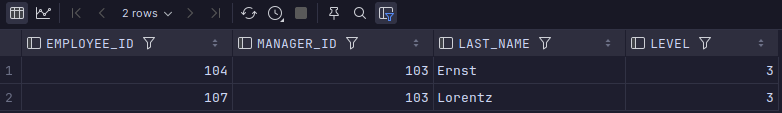
\includegraphics[width=1\linewidth]{../ue3_2_2.png}
	\caption{Aufgabe 2 Ergebnisse 3}
\end{figure}

\begin{figure}[H]
	\centering
	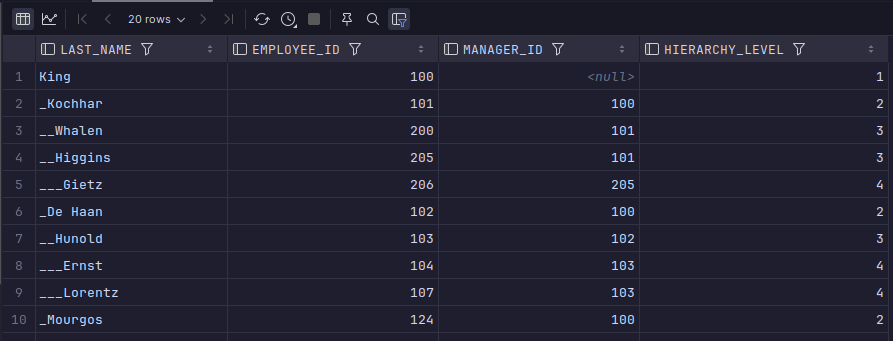
\includegraphics[width=1\linewidth]{../ue3_2_3.png}
	\caption{Aufgabe 2 Ergebnisse 4}
\end{figure}

\pagebreak

\section{Hierarchische Abfragen - Sakila}

\subsection{SQL Queries}

\inputminted{sql}{../ue3_3.sql}

\subsection{Ergebnisse}

\begin{figure}[H]
	\centering
	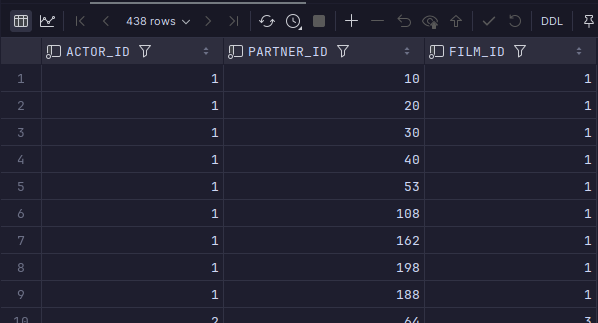
\includegraphics[width=1\linewidth]{../ue3_3a.png}
	\caption{Aufgabe 3 Ergebnisse 1}
\end{figure}

\begin{figure}[H]
	\centering
	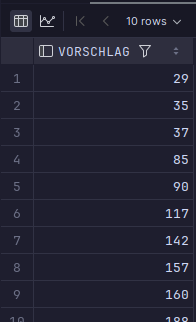
\includegraphics[width=0.3\linewidth]{../ue3_3b.png}
	\caption{Aufgabe 3 Ergebnisse 2}
\end{figure}

\pagebreak

\section{Analytische Abfragen - Sakila}

\subsection{SQL Queries}

\inputminted{sql}{../ue3_4.sql}

\subsection{Ergebnisse}

\begin{figure}[H]
	\centering
	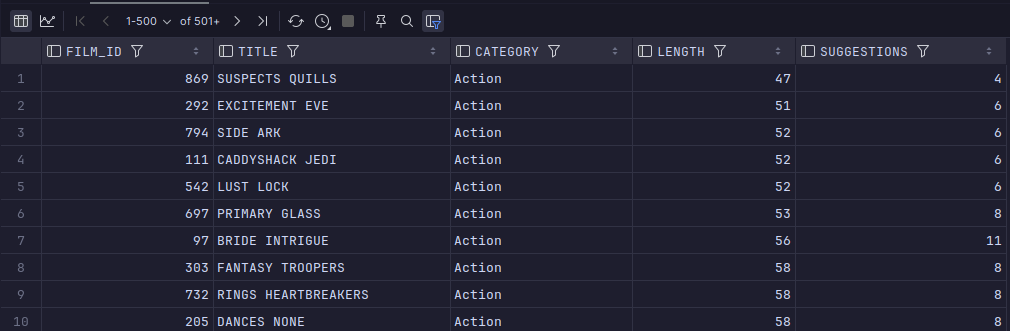
\includegraphics[width=1\linewidth]{../ue3_4_1.png}
	\caption{Aufgabe 4 Ergebnisse 1}
\end{figure}

\begin{figure}[H]
	\centering
	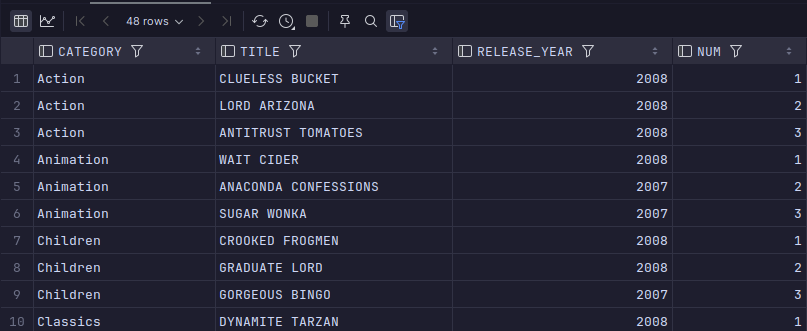
\includegraphics[width=1\linewidth]{../ue3_4_2.png}
	\caption{Aufgabe 4 Ergebnisse 2}
\end{figure}

\begin{figure}[H]
	\centering
	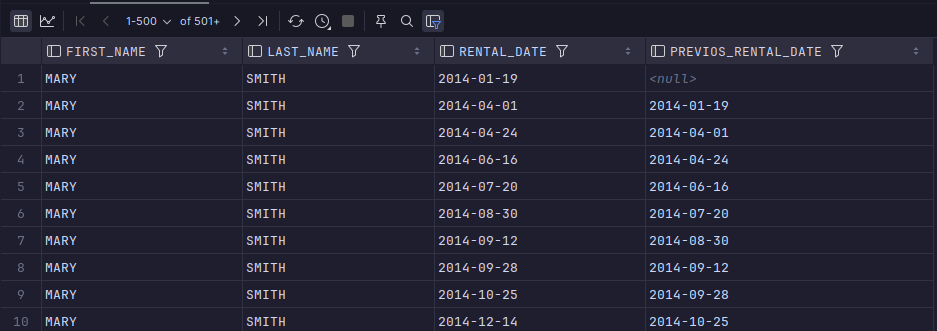
\includegraphics[width=1\linewidth]{../ue3_4_3a.png}
	\caption{Aufgabe 4 Ergebnisse 3}
\end{figure}

\begin{figure}[H]
	\centering
	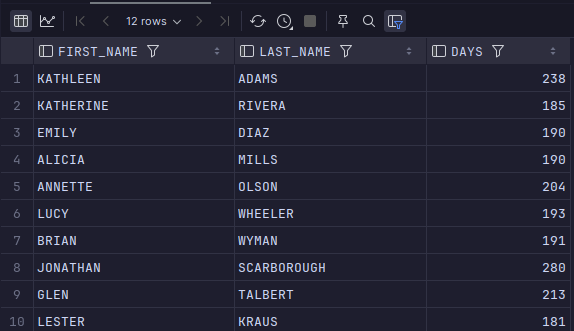
\includegraphics[width=1\linewidth]{../ue3_4_3b.png}
	\caption{Aufgabe 4 Ergebnisse 4}
\end{figure}

\pagebreak

\section{LISTAGG - Sakila}

\subsection{SQL Queries}

\inputminted{sql}{../ue3_5.sql}

\subsection{Ergebnisse}

\begin{figure}[H]
	\centering
	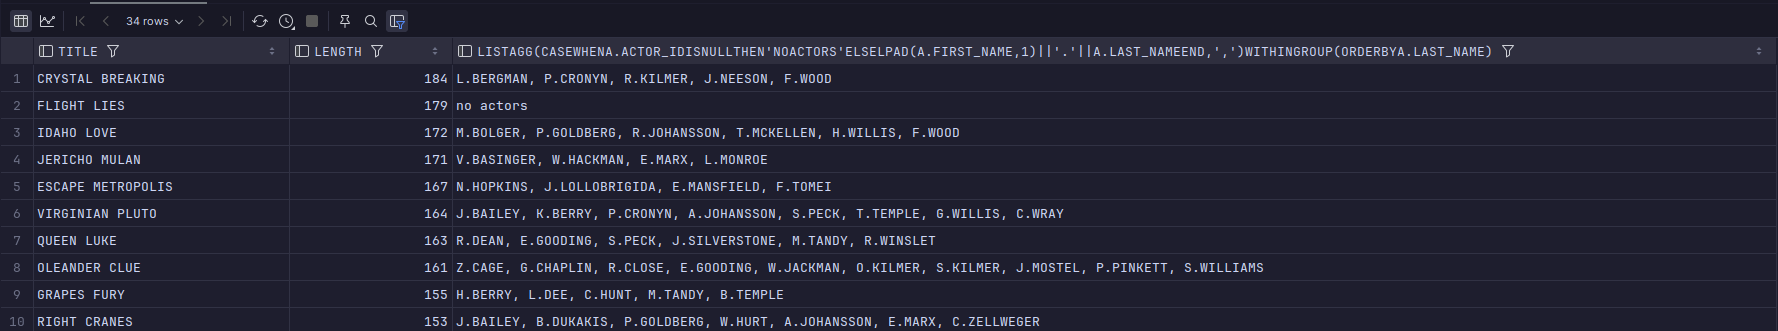
\includegraphics[width=1\linewidth]{../ue3_5_1.png}
	\caption{Aufgabe 5 Ergebnisse 1}
\end{figure}

\begin{figure}[H]
	\centering
	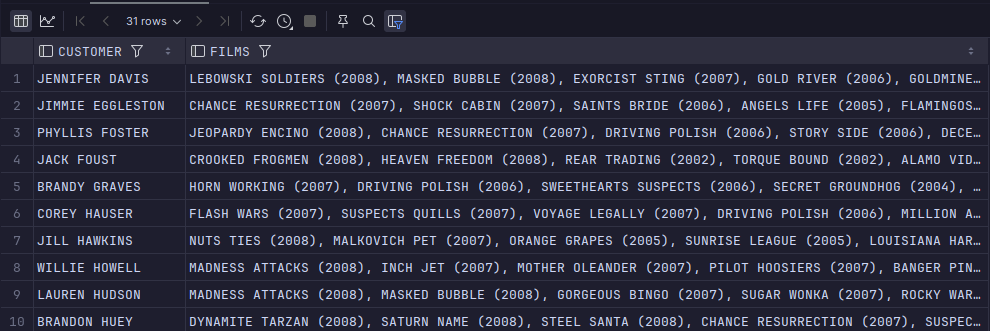
\includegraphics[width=1\linewidth]{../ue3_5_2.png}
	\caption{Aufgabe 5 Ergebnisse 2}
\end{figure}

\pagebreak

\section{Materialisierte Sichten - Sakila}

\subsection{SQL Queries}

\inputminted{sql}{../ue3_6.sql}

\subsection{Ergebnisse}

\begin{figure}[H]
	\centering
	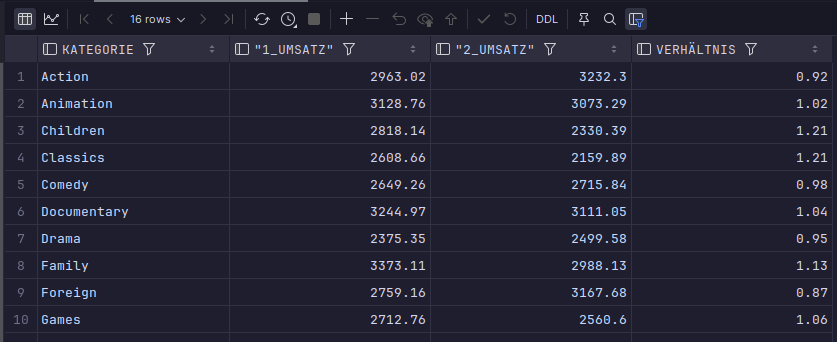
\includegraphics[width=1\linewidth]{../ue3_6.png}
	\caption{Aufgabe 6 Ergebnisse}
\end{figure}

\end{document}